\chapter{实验结果与分析}
\label{cha:res}

实验将抓取的高性能应用的IO Trace通过映射和垃圾回收机制转换为对开放通道SSD内部结构操作,并使用liblightnvm对其进行直接读写,最后通过吞吐量、映射表修改次数、擦除次数和写放大系数等性能指标评价优化方法的优劣。此外,实验还研究了不同优化方法下剩余空间大小对IO性能的影响,以及超级块方法中超级块参数的影响。本章中的PM\_GCL,PM\_GCC和SBM\_GCL分别指页映射-贪心垃圾回收策略、页映射-连续空间垃圾回收策略和超级块映射-贪心垃圾回收策略。

\section{实验环境}
由于硬件条件限制,本章中所有实验均在开放通道SSD的模拟器上进行。因此,下文的"硬件环境"包括运行模拟器的设备的硬件环境,模拟器以及模拟出的开放通道SSD的基本参数。下文的"软件环境"包括模拟器使用的Linux内核版本与相关用户态库的信息。
\subsection{硬件环境}
实验使用一台Linux服务器运行模拟器,服务器的CPU为Intel(R) Xeon(R) CPU E5-2620 v2 @ 2.10GHz,内存大小16GB。模拟器使用https://github.com/DFC-OpenSource/qemu-ox 提供的支持模拟开放通道SSD的qemu虚拟机。除特殊说明外,实验使用的模拟开放通道SSD设备基本信息如下表:
\begin{table}[htb]
    \centering
    \begin{minipage}[t]{0.8\linewidth}
    \caption[开放通道SSD的基本信息]{开放通道SSD的基本信息}
    \label{tab:res_ocssd_geo}
      \begin{tabularx}{\linewidth}{cY}
        \toprule[1.5pt]
        {\heiti 参数名} & {\heiti 数值} \\\midrule[1pt]
        Channel数量 & 8\\
        每个Channel的Lun数量 & 4\\
        每个Lun的Block数量 & 64\\
        每个Block的Page数量 & 8\\
        每个Page的Sector数量 & 4\\
        Plane数量 & 2\\
        每个Sector能够容纳的数据量 & 4096 Byte\\
        每个Page能够容纳的数据量 & 32768 Byte\\ 
        \bottomrule[1.5pt]
    \end{tabularx}
\end{minipage}
\end{table}
\subsection{软件环境}
模拟器运行的Linux内核版本为4.17.0,编译时打开了CONFIG\_BLK\_DEV\_NVME,CONFIG\_NVM,CONFIG\_NVM\_DEBUG,CONFIG\_NVM\_PBLK选项以提供对开放通道SSD的驱动支持。实验使用的用于直接操作开放通道SSD设备的用户态库liglightnvm版本为master@ba201ca。

\section{IO吞吐量}
图\ref{fig:res_iototal}和表\ref{tab:res_iototal}展示了不同优化方法重放高性能应用的IO Trace时的IO吞吐量。可以发现,在重放LAMMPS和MACDRP两种应用的Trace时,与页映射-贪心垃圾回收方法相比,页映射-连续空间垃圾回收的IO吞吐量显著偏低,而超级块映射-贪心垃圾回收的方法IO吞吐量与之相接近。
\begin{figure}[H]
    \centering
    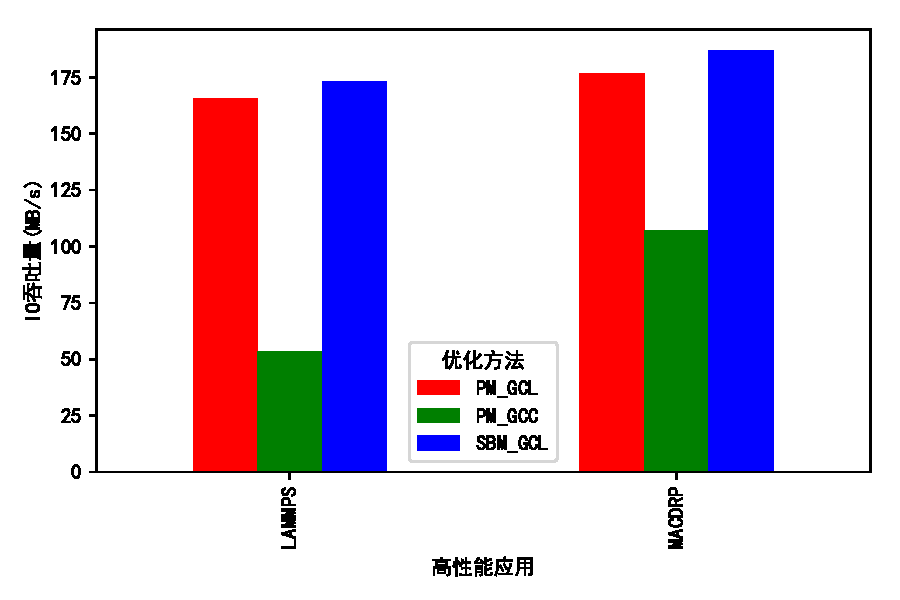
\includegraphics[width=0.8\textwidth]{iothroughput.pdf}
    \caption{不同优化方法的IO吞吐量}
    \label{fig:res_iototal}
\end{figure}

\begin{table}[htbb]
    \centering
    \begin{minipage}[t]{0.8\linewidth}
    \caption[不同优化方法的IO吞吐量(MB/s)]{不同优化方法的IO吞吐量(MB/s)}
    \label{tab:res_iototal}
    \begin{tabularx}{\linewidth}{cYYY}
        \toprule[1.5pt]
        \multirow{2}{*}{\heiti{高性能应用}} & \multicolumn{3}{c}{\heiti{优化方法}}  \\ \cmidrule(l){2-4} 
                     & PM\_GCL & PM\_GCC & SBM\_GCL \\ \midrule[1pt]
                     LAMMPS &65.448&53.217    & \textbf{173.116}    \\
                     MACDRP    & 176.768 &107.184    & \textbf{186.747}    \\ \bottomrule[1.5pt]
        \end{tabularx}
    \end{minipage}
\end{table}

为了更细致地刻画几种方法在IO吞吐量上的表现,以下从平均IO吞吐量在重放过程中的变化和单次IO吞吐量的分布来分析不同方法下的IO过程。
图\ref{fig:res_ioavg}反映了重放过程中平均IO吞吐量随IO请求总量的变化过程。
三种方法在早期均倾向于占据未分配的空间进行写入,当SSD上几乎所有空间均无法写入时开始进行垃圾回收,平均IO吞吐量开始下降并最终稳定到某个水平。对于页映射-贪心垃圾回收方法和超级块映射-贪心垃圾回收方法,二者每次进行垃圾回收均只需要回收一个块或者数个块的空间,且单次回收空间量的上限被本次IO的写入量所限制,故每次垃圾回收需要重新写入的脏页数量和需要擦除的块数量均相对较小。在这种机制下SSD上可直接写入的空间会长期维持在较低水平,每次写入均需进行小规模的垃圾回收,平均IO吞吐量受单次IO的影响较小。对于页映射-连续空间垃圾回收方法,由于空闲区域写满后需要在全盘范围内进行一次垃圾回收,需要擦除的块和重写的脏页遍布整个SSD,因此若当前IO无需进行垃圾回收则能够以顺序写的方式保持较高速率写入,若需要进行垃圾回收则要等待较长时间导致平均IO吞吐量突然下降。
连续空间垃圾回收每次均需要将当前有效数据重新写入,而贪心垃圾回收则未必。故连续空间垃圾回收的总成本更高,平均IO吞吐量更低,且在写入有效数据更多的LAMMPS的Trace上表现更差;而贪心垃圾回收的表现不受Trace写入的有效数据量影响。

\begin{figure}[H]
    \centering
    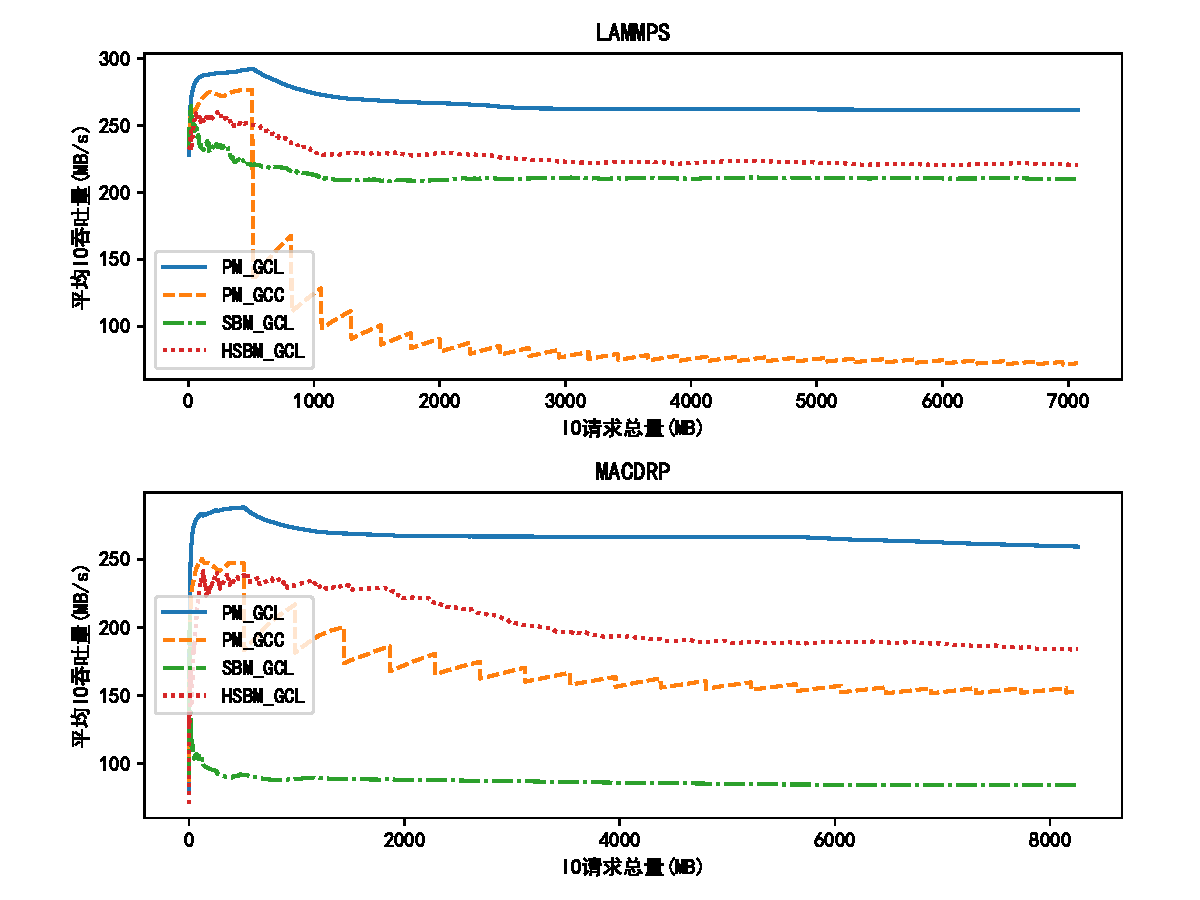
\includegraphics[width=0.8\textwidth]{avgiothp.pdf}
    \caption{平均IO吞吐量在重放过程中随IO请求总量的变化}
    \label{fig:res_ioavg}
\end{figure}

图\ref{fig:res_ioingle}按照IO请求发出的先后顺序绘制了每次IO的吞吐量。两种使用贪心垃圾回收策略的方法的单次IO吞吐量分布类似。连续空间垃圾回收方法尽管有大量写请求均能按照连续写速率(约300MB/s)写入,但每次发生垃圾回收时需要的开销过大,导致发生垃圾回收的写请求吞吐量接近0,整体吞吐量表现反而不如贪心垃圾回收方法。

\begin{figure}[H]
    \centering
    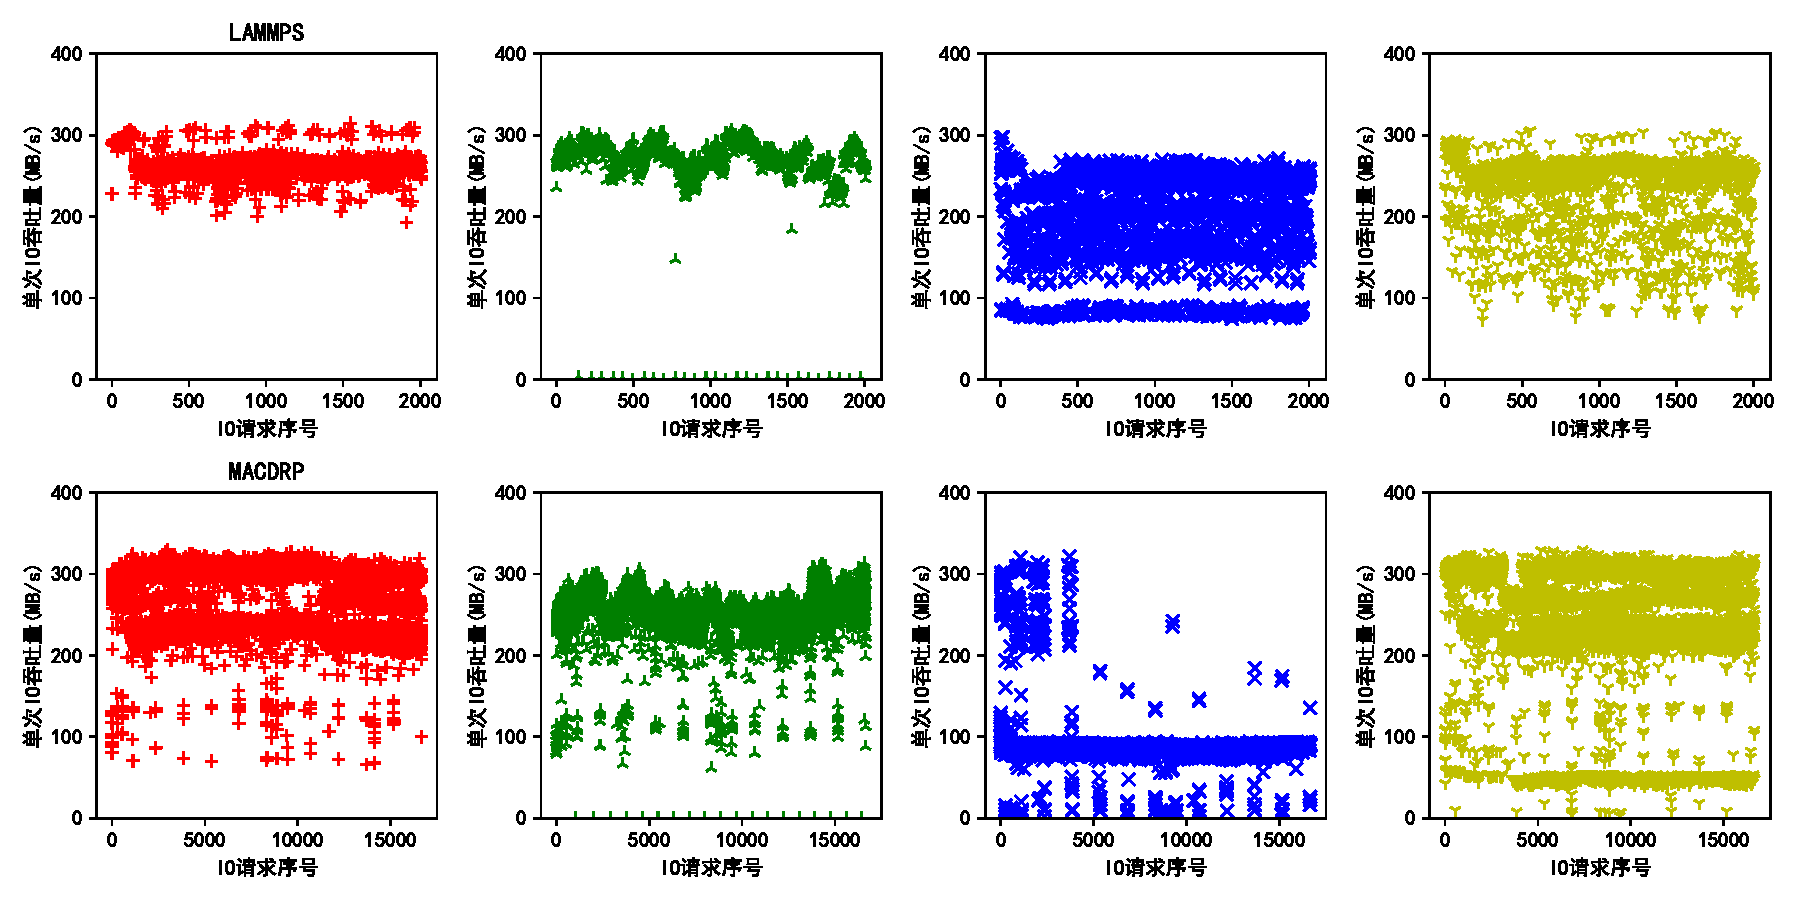
\includegraphics[width=0.8\textwidth]{singleiothp.pdf}
    \caption[不同优化方法在重放过程中的单次IO吞吐量]{不同优化方法在重放过程中的单次IO吞吐量,红色、绿色、蓝色分别代表页映射-贪心垃圾回收方法、页映射-连续空间垃圾回收方法和超级块映射-贪心垃圾回收方法}
    \label{fig:res_ioingle}
\end{figure}

\section{映射表开销}

超级块映射方法与页映射方法相比,其显著优势在于映射表占用空间更小,且维护映射表需要的成本更低。在映射表每个表项使用64位整形数存储对应的物理地址,占用空间为8Byte的条件下,对于实验用表\ref{tab:res_ocssd_geo}所示设备,页映射需要的映射表空间为$8\times 4\times 64\times 8\times 8\mathrm{Byte}=128\mathrm{KB}$,占设备全部可用空间的$1/4096$。而使用包含一个块的超级块映射,映射表所需空间为$8\times 4\times 64\times 8\mathrm{Byte}=16\mathrm{KB}$,占比仅为$1/32768$。由于超级块映射的表项更少,维护起来也更加简单。

\begin{figure}[H]
    \centering
    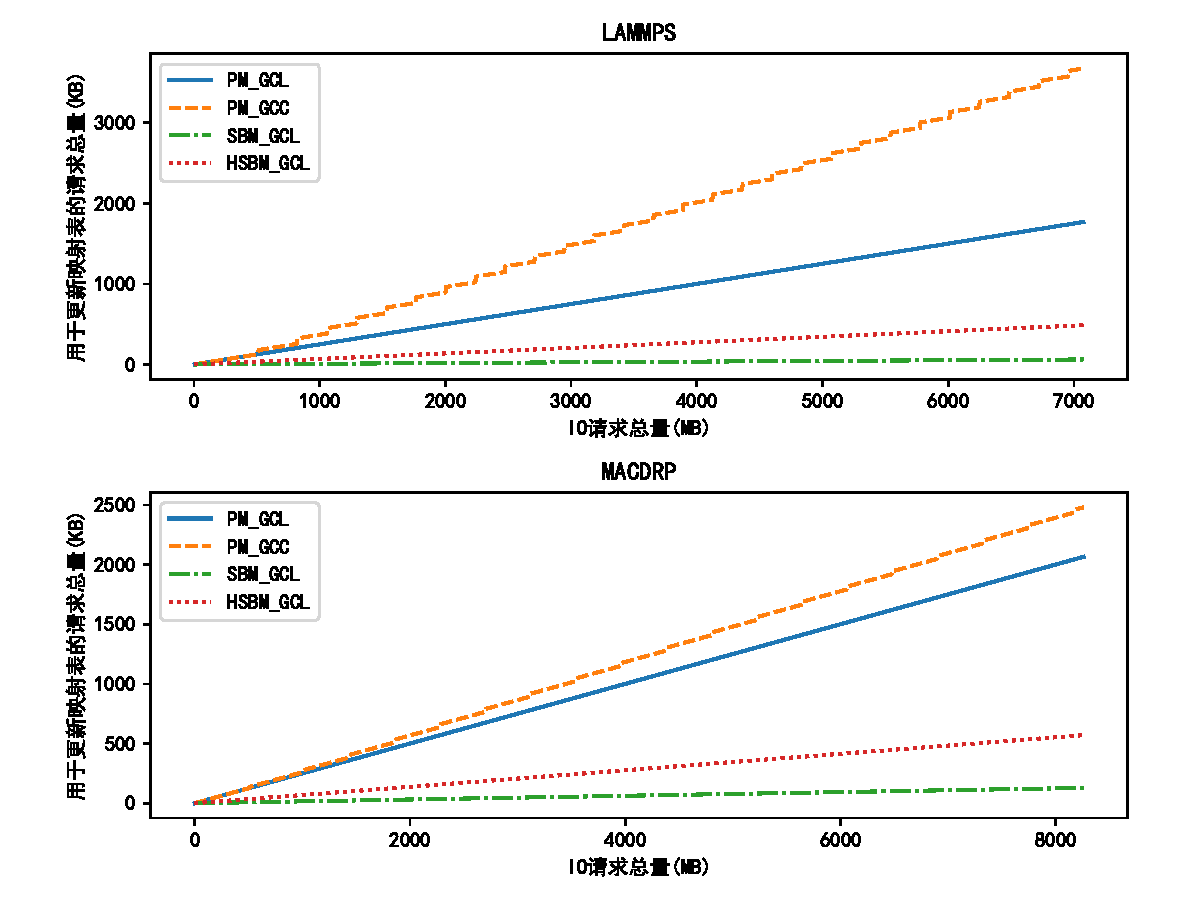
\includegraphics[width=0.8\textwidth]{mapupdateio.pdf}
    \caption{用于更新映射表的请求总量在重放过程中随IO请求总量的变化}
    \label{fig:res_mapupdate}
\end{figure}

如图\ref{fig:res_mapupdate},在LAMMPS负载下,页映射-贪心垃圾回收方法和页映射-连续空间垃圾回收方法每完成7G的IO写请求分别需要传输1768KB和3805KB的数据用于映射表更新,而超级块映射方法仅需要221KB;在MACDRP负载下,这一维护成本对于两种页映射方法分别为每8GB 2065KB和2477KB,对于超级块映射方法则仅为每8GB 259KB。

\section{擦除次数与写放大系数}

在设备自身的读写性能一定的情况下,映射算法和垃圾回收算法造成的擦除与写放大是影响整体吞吐量的最主要因素。这里以IO请求总量为变量,分析重放过程中擦除次数与写放大系数的变化。这里擦除次数定义为从重放开始擦除的Block总数,写放大系数定义为$\dfrac{\text{向设备写入的总数据量}}{\text{完成的写请求总数据量}}$。

\begin{figure}[H]
    \centering
    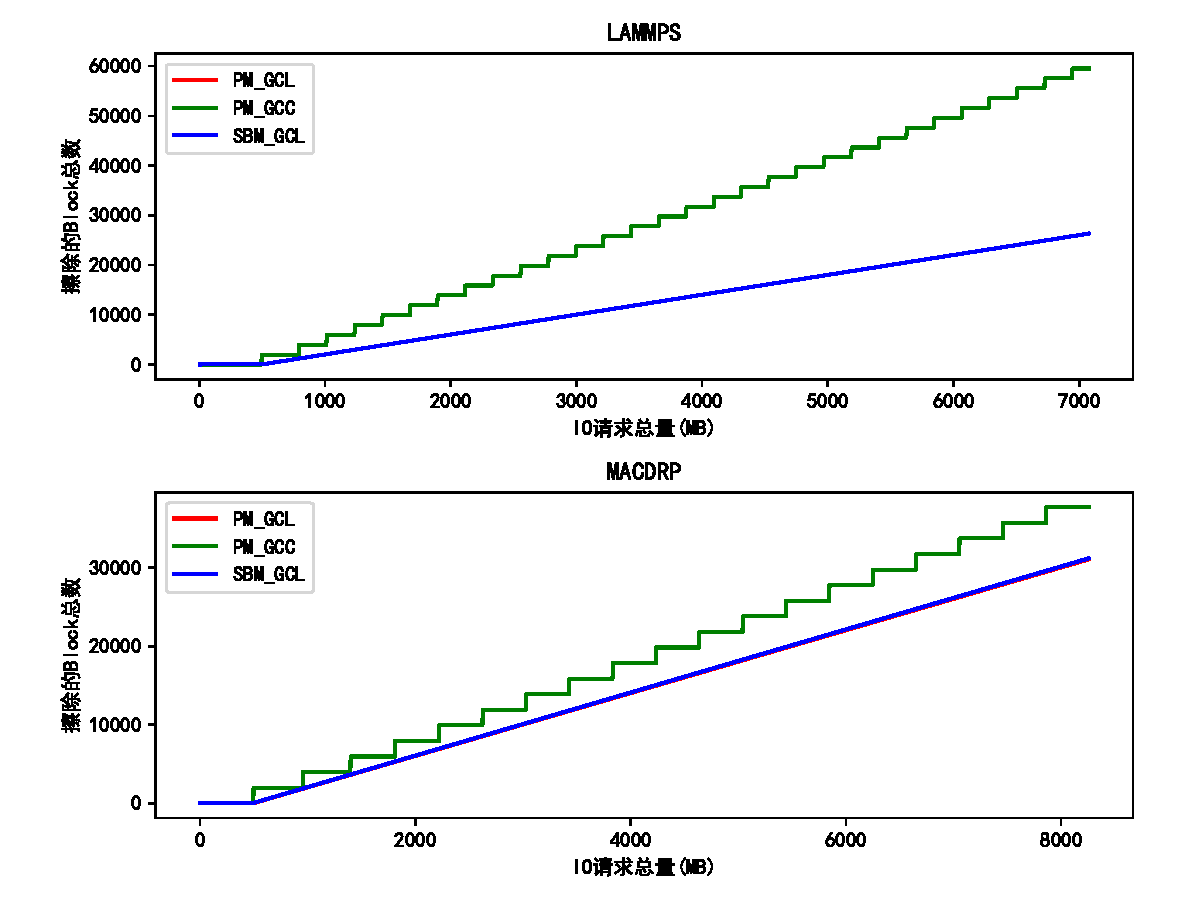
\includegraphics[width=0.8\textwidth]{eraseblk.pdf}
    \caption{擦除的Block数在重放过程中随IO请求总量的变化}
    \label{fig:res_erasecount}
\end{figure}

如图\ref{fig:res_erasecount},页映射-贪心垃圾回收方法和超级块映射-贪心垃圾回收方法的擦除次数与IO请求总量的关系几乎完全相同且近似线性变化。这是因为两种方法每次进行垃圾回收需要擦除的块数均受到当前IO写入量的控制,两种高性能应用每次IO请求的写入量相对恒定,与方法本身无关;两种方法下设备可直接写入的空间稳定在较低水平,每次写入均需要进行小范围的垃圾回收。页映射-连续空间垃圾回收方法的擦除次数呈现阶梯状变化,且写入有效数据较多的LAMMPS应用下擦除次数变化的间隔更小,原因是该方法每次垃圾回收后会腾出设备上除已写入有效数据的所有空间用于写入,待这段空间写满后才会再次进行垃圾回收,故两次垃圾回收之间有较大间隔;写入的有效数据越多,腾出的空间越少,垃圾回收间隔越小。

\begin{figure}[H]
    \centering
    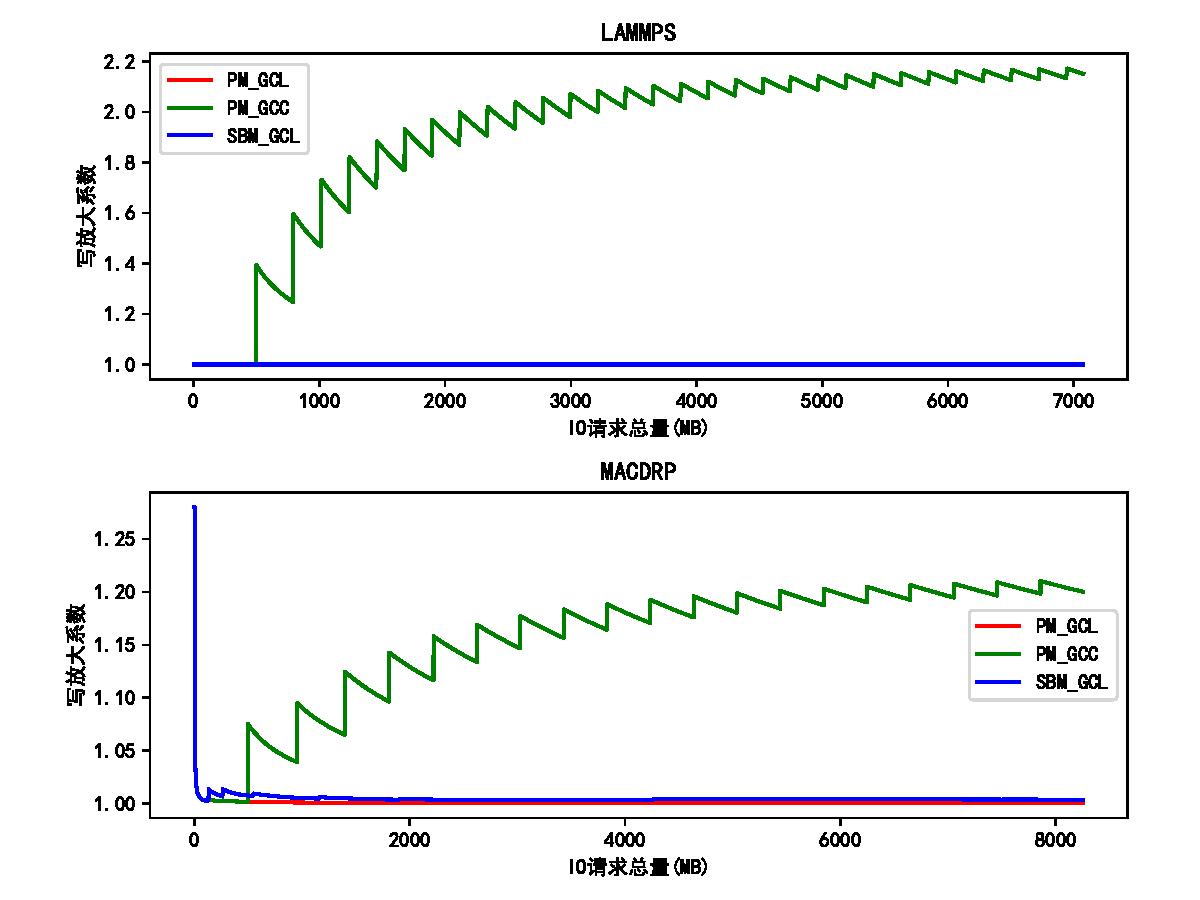
\includegraphics[width=0.8\textwidth]{writeampio.pdf}
    \caption{写放大系数在重放过程中随IO请求总量的变化}
    \label{fig:res_writeamp}
\end{figure}

如图\ref{fig:res_writeamp},两种贪心垃圾回收方法的写放大系数随着写入量增加很快稳定在1左右,而连续空间垃圾回收方法的写放大系数逐渐增加并维持在大于1的水平。两种应用的写请求起始位置绝大部分都按页对齐,一次连续写入的量大部分能覆盖一个或者多个Block,覆盖写的起始位置和大小与第一次写请求往往相同,因此每次覆盖写都会造成大量的整块Block中的数据无效。对于贪心垃圾回收,其只需要对相应块进行清除操作而无需重新写入大量脏页;对于连续空间垃圾回收,已写入的所有脏页均需要读出后重新写入,造成写放大系数偏高。

\section{负载均衡}

这里通过可视化设备上每个Page/Block执行写操作/擦除操作的次数比较不同方法的负载均衡情况。

\begin{figure}[H]
    \centering
    \subcaptionbox{重放LAMMPS时的负载分布}
      {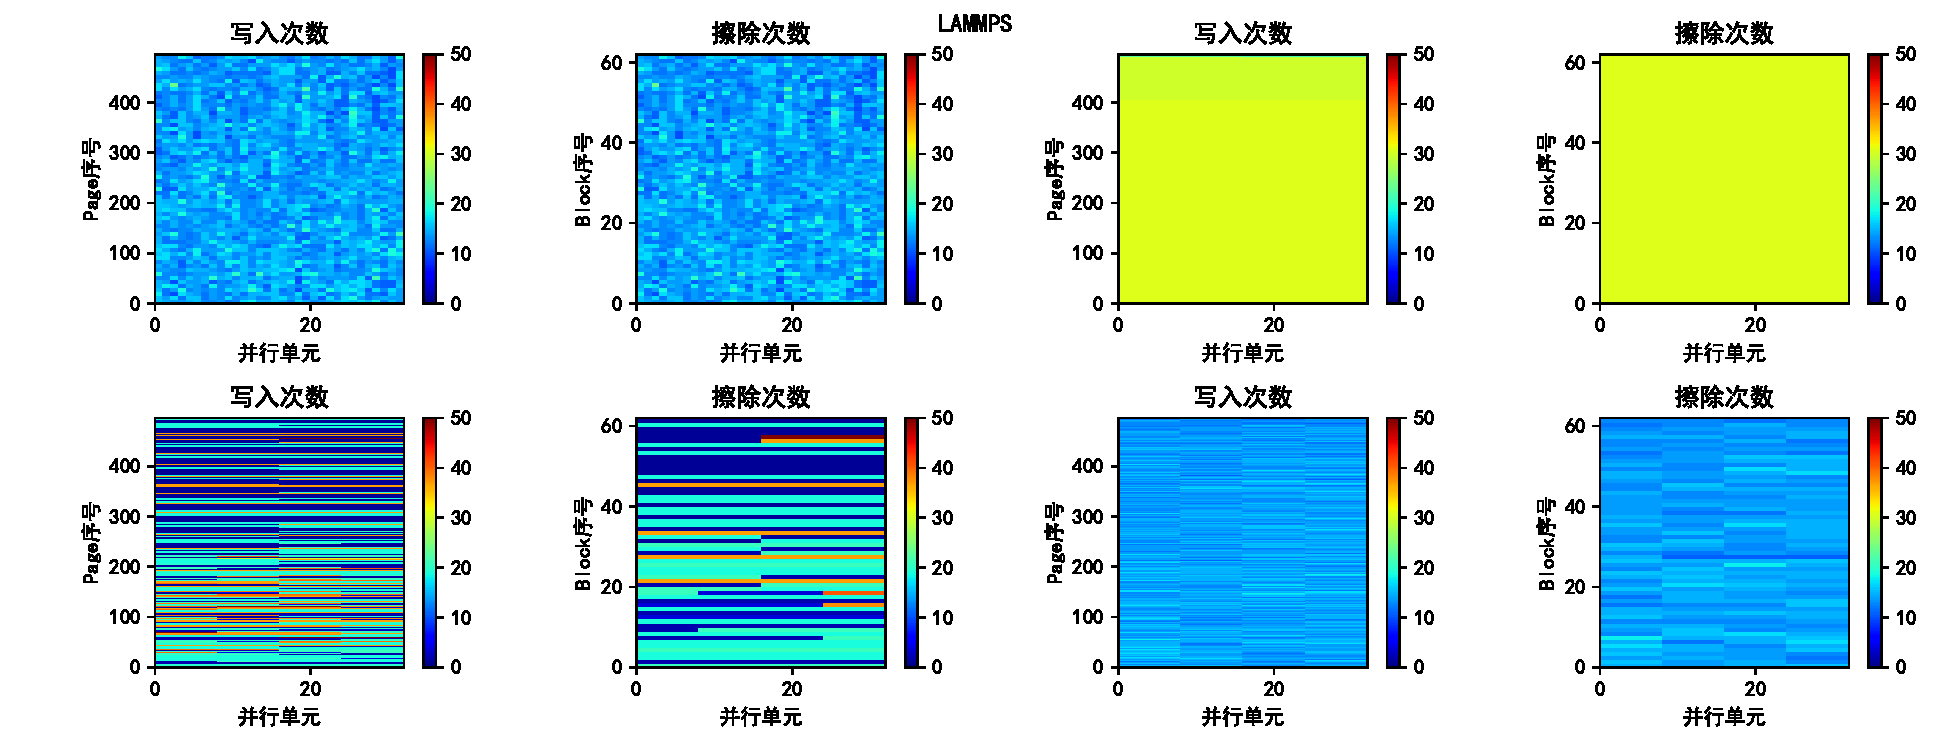
\includegraphics[width=0.8\textwidth]{heatmap_lammps.pdf}}
    \vspace{4em}
    \subcaptionbox{重放MACDRP时的负载分布}
        {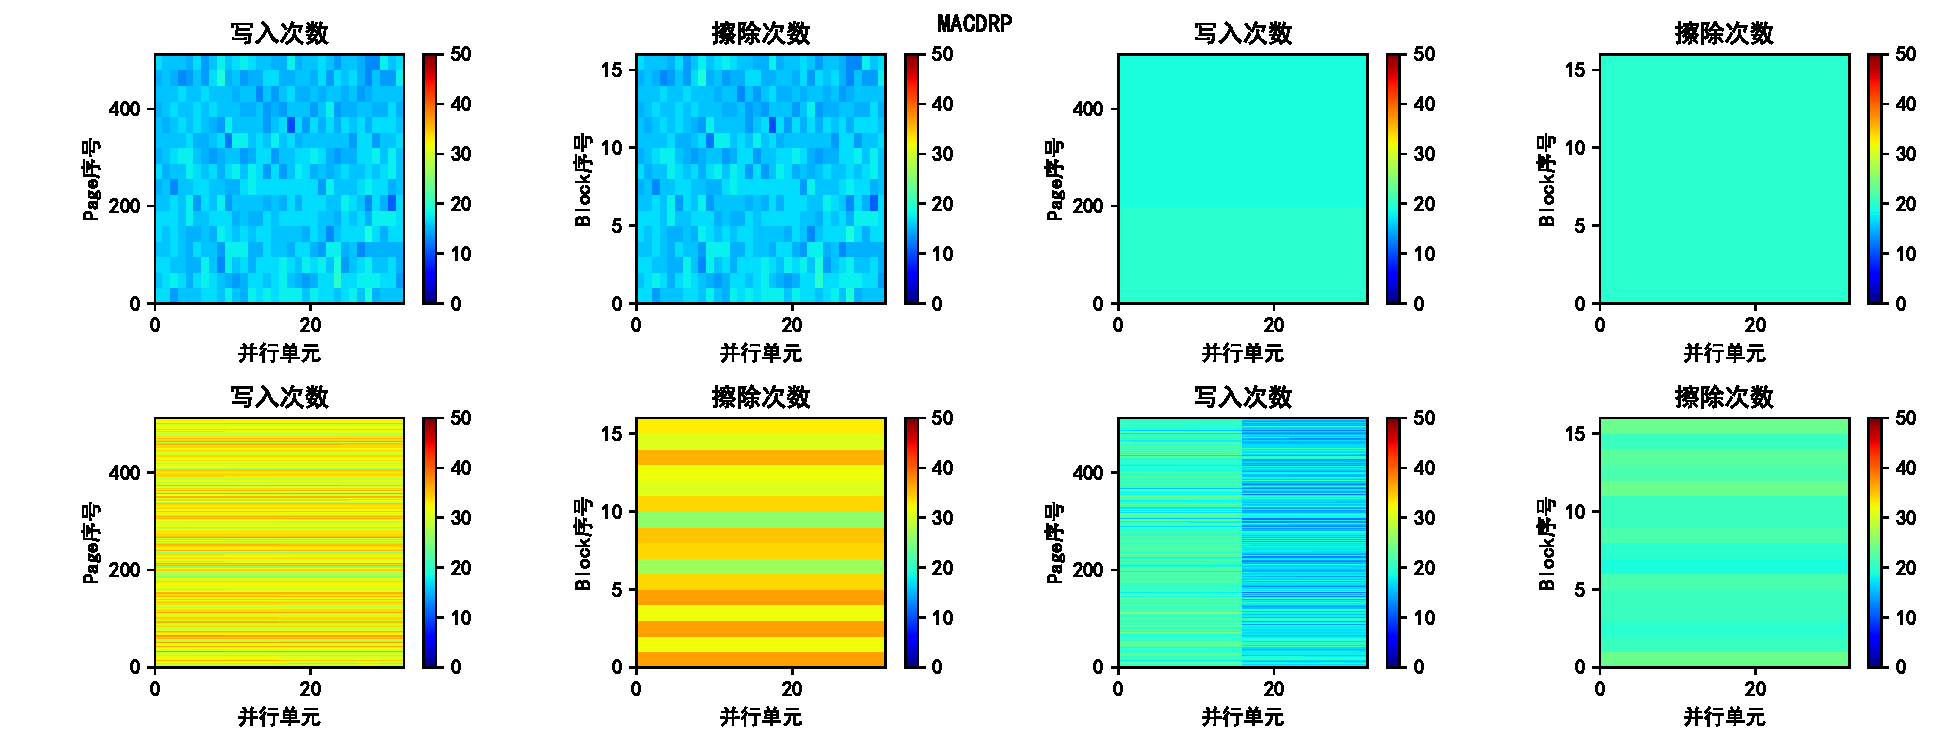
\includegraphics[width=0.8\textwidth]{heatmap_macdrp.pdf}}
    \caption[负载分布图]{负载分布图,每种应用的负载分布图的左上、右上、左下、右下各2张图分别代表页映射-贪心垃圾回收方法、页映射-连续空间垃圾回收方法、未改进负载均衡的超级块映射-贪心垃圾回收方法和改进后的该方法的写、擦除次数分布}
    \label{fig:res_heatmap}
\end{figure}

如图\ref{fig:res_heatmap},页映射-连续空间垃圾回收方法的负载均衡效果最好,所有位置的写入次数和擦除次数均几乎相同,原因是该方法在设备的几乎所有页被写入后才进行垃圾回收,而垃圾回收会对设备的所有块进行擦除,整个设备不断循环全部写入-全部擦除的过程。改进前的超级块映射-贪心垃圾回收负载均衡效果较差,因为在所有超级块均被写入并建立映射关系后,当前发生覆盖写的超级块中的脏页会在与写请求合并后就地重新写入擦除后的该块,映射关系不发生改变,导致被擦除的块的选择与写请求的起始位置有关。改进后的方法强制要求每次覆盖写选择另一位置的超级块写入,从而改善了负载均衡。

\section{设备容量的影响}

设备容量的大小可能对映射表维护和垃圾回收的开销产生影响。这里通过改变每个Lun含有的Block数量改变设备容量,使得设备容量分别为写入的有效数据量的2倍、4倍和8倍,观察这一变化对吞吐量、映射表修改次数、擦除次数和写放大系数等性能指标的影响。

\begin{figure}[H]
    \centering
    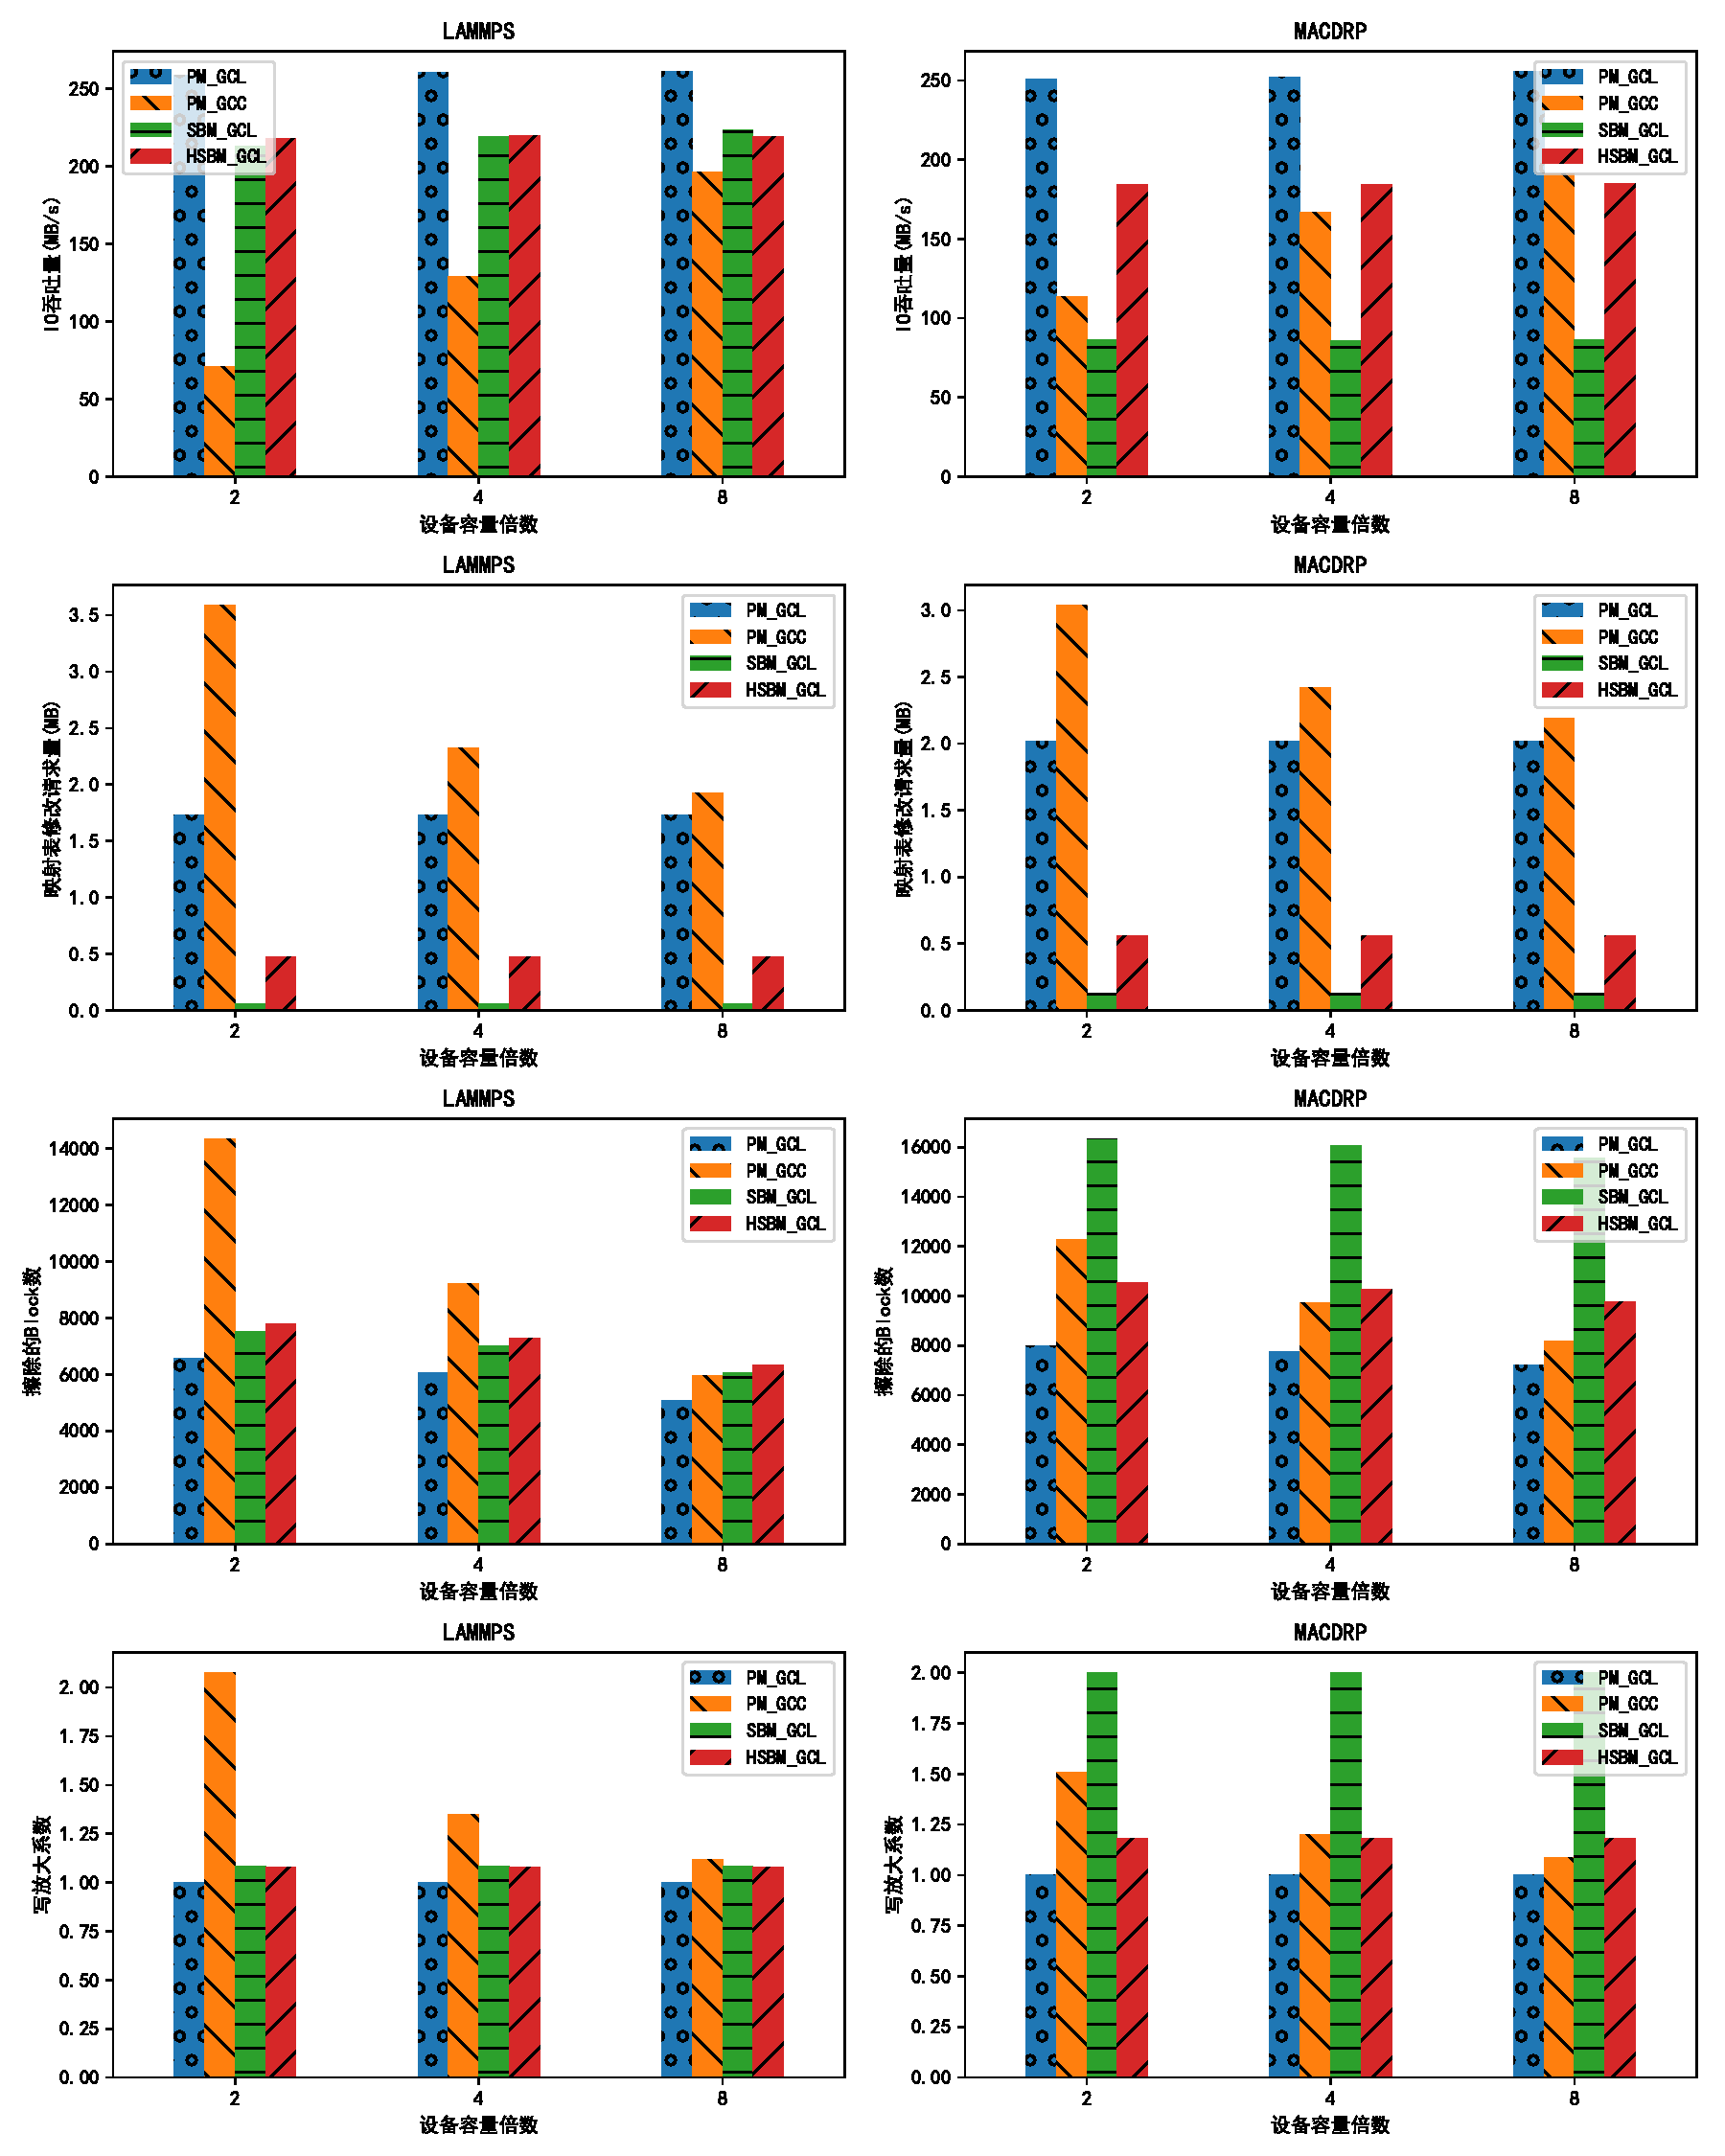
\includegraphics[width=0.8\textwidth]{disksize.pdf}
    \caption{设备容量对各项性能指标的影响}
    \label{fig:res_disksize}
\end{figure}

如图\ref{fig:res_disksize},页映射-贪心垃圾回收和超级块映射-贪心垃圾回收方法在设备容量增大时性能提高很小或基本不变,原因是设备容量增大只能延长两种方法第一次进行垃圾回收前连续写入的阶段,而这一阶段虽然无需进行垃圾回收,性能最好,但持续时间占整个重放过程的比例很低。达到稳定状态后两种方法都只在设备上维持很少的可用空间,开销与设备容量无关。对于页映射-连续空间垃圾回收方法,设备容量的增大增加了两次垃圾回收的间隔,尽管一次垃圾回收需要擦除的块数量更多,但垃圾回收次数减少和写放大系数降低带来的好处更大,故该方法在设备容量增大时性能提高较多。

\section{超级块大小的选择}

超级块映射涉及到设置为超级块设置合适的大小。较大的超级块能够显著减小映射表体积和维护成本,但发生覆盖写时需要擦除和重新写入的脏页数量也更多;较小的超级块则反之。这里通过调整超级块的大小为1、2、4、8个块,比较不同设置下超级块映射-贪心垃圾回收方法的性能指标。

\begin{figure}[H]
    \centering
    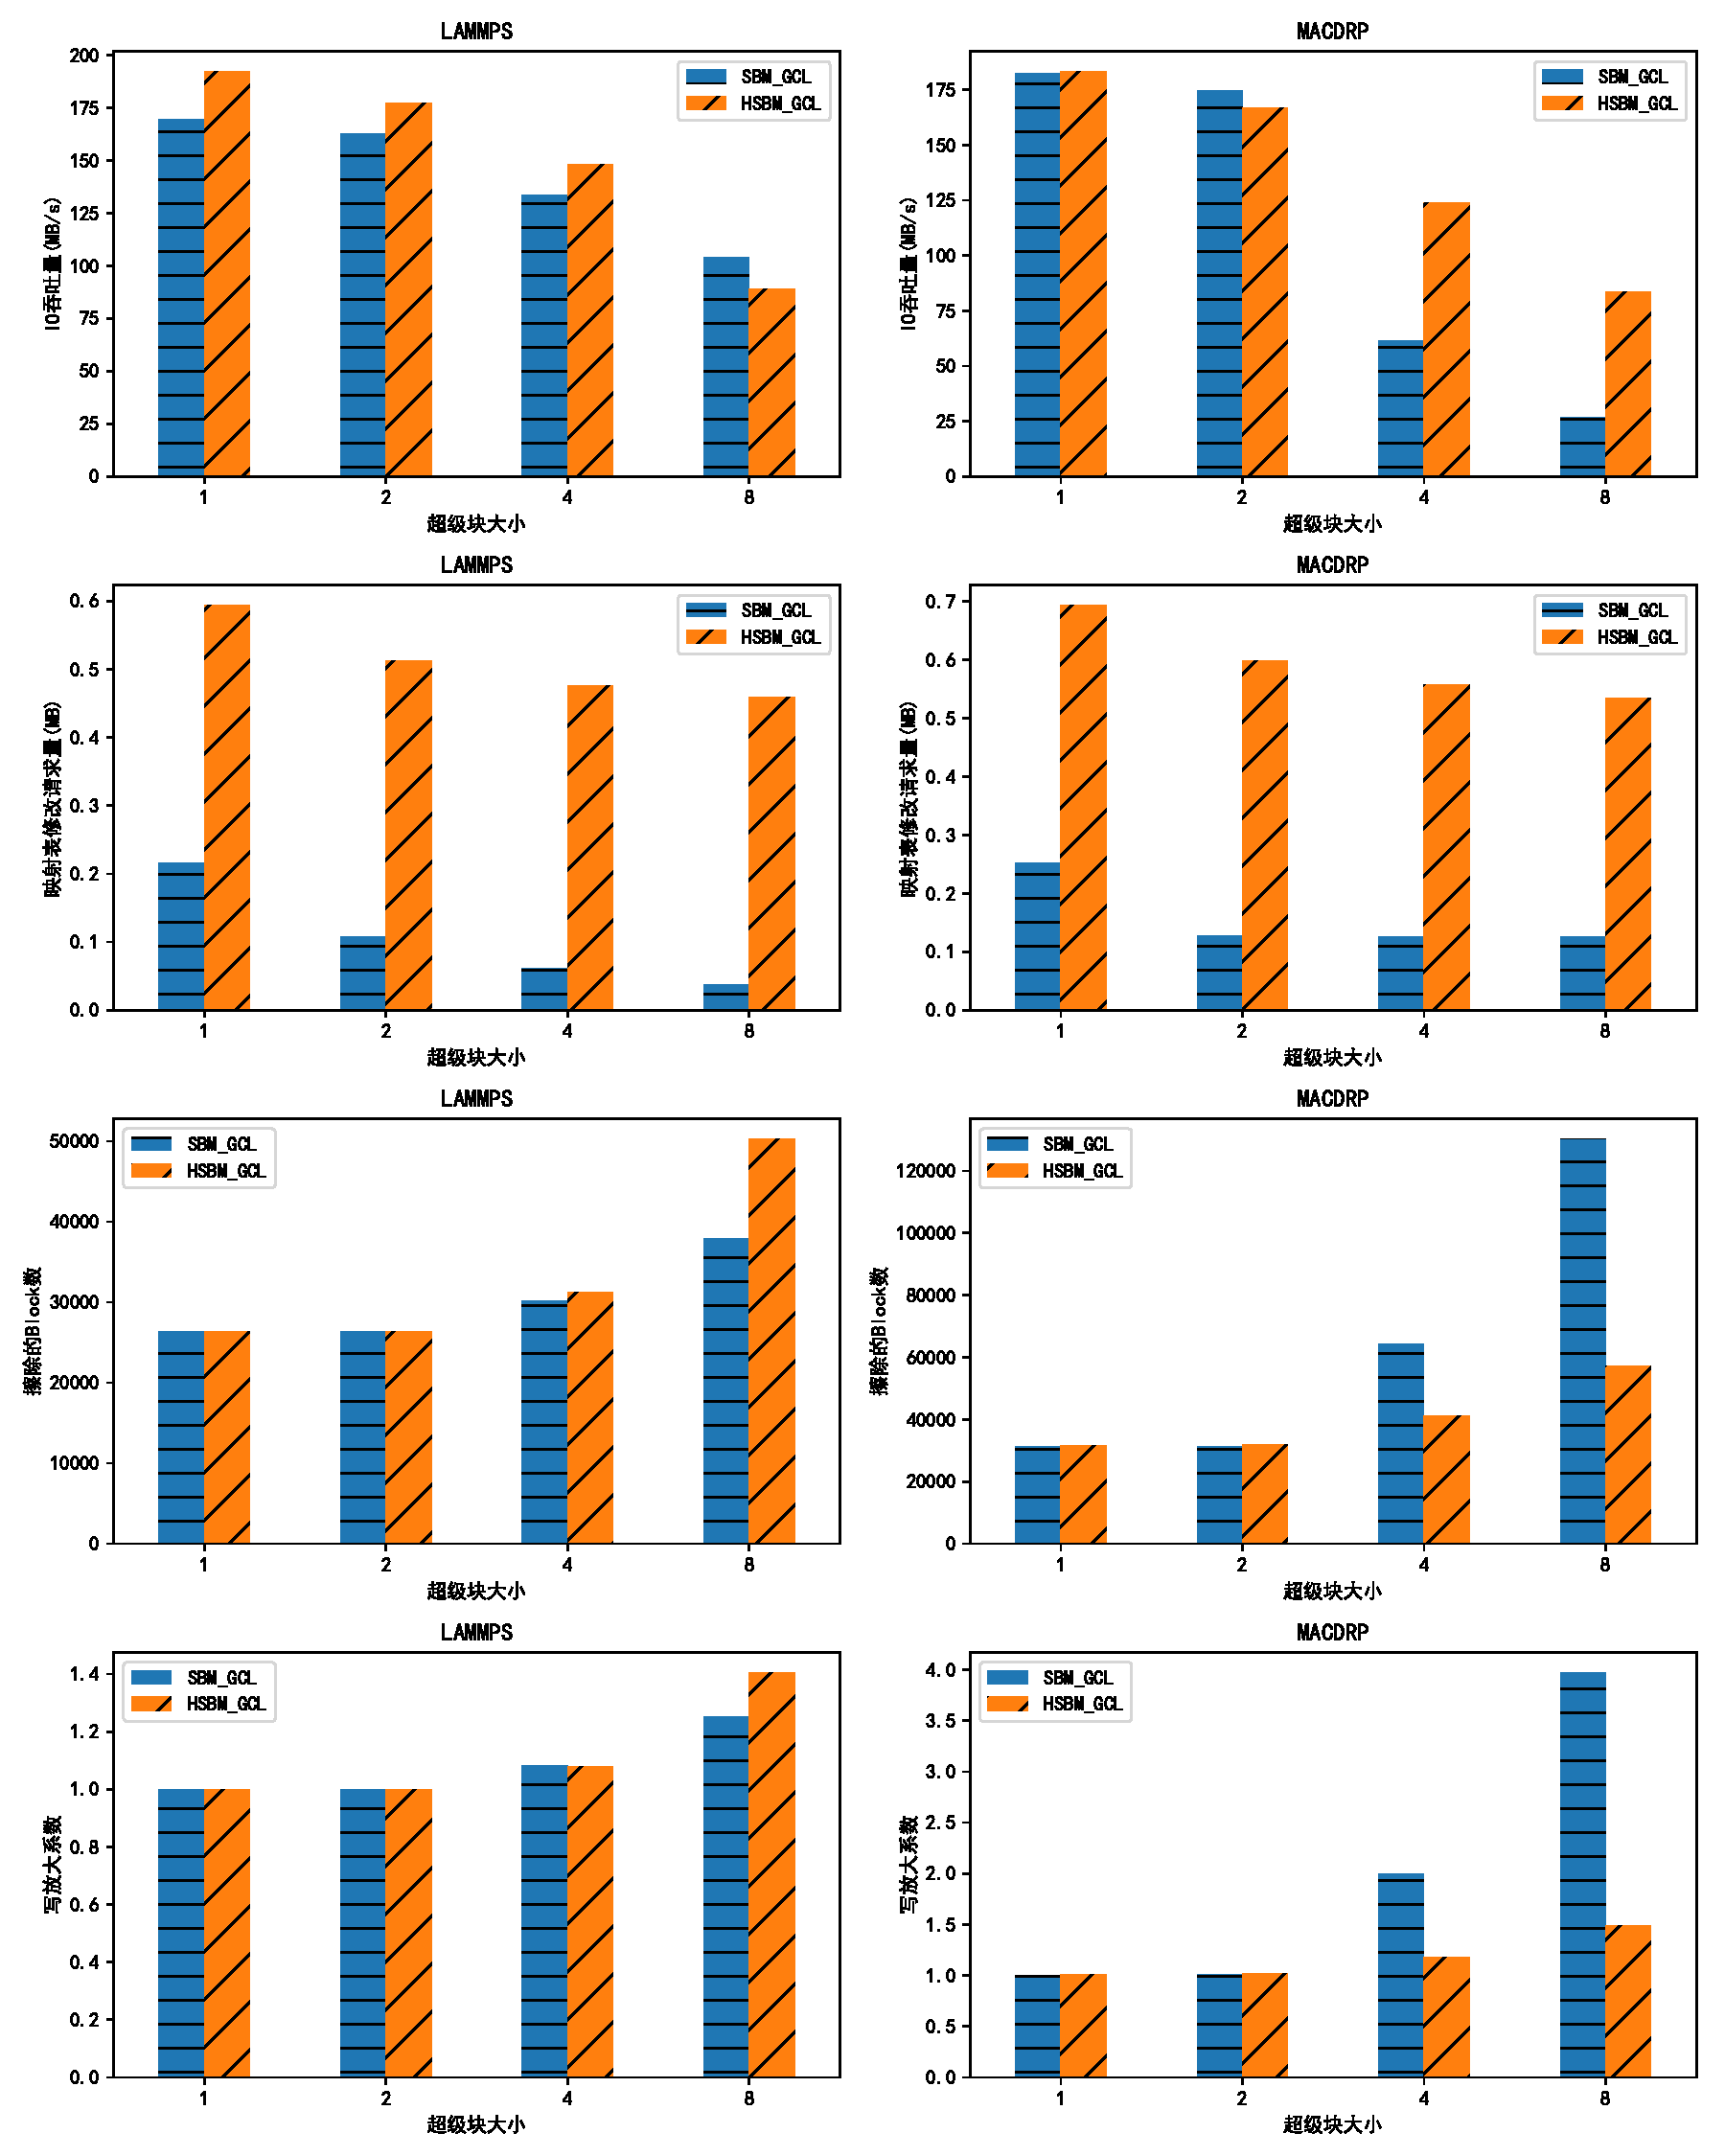
\includegraphics[width=0.8\textwidth]{sbsize.pdf}
    \caption{超级块大小对各项性能指标的影响}
    \label{fig:res_sbsize}
\end{figure}

如图\ref{fig:res_sbsize},超级块大小从1增加到2时,吞吐量有很小的下降,擦除次数和写放大系数几乎不改变,而映射表维护次数下降了接近50\%。超级块大小继续从2增加到4和8时,对于LAMMPS应用,吞吐量仍是小幅下降,擦除次数和写放大系数上升很小,映射表维护次数则继续随超级块大小翻倍而减半;对于MACDRP应用,吞吐量下降幅度较大,擦除次数和写放大系数大幅上升,映射表维护次数的变化与LAMMPS类似。其中的原因是LAMMPS一次连续写入的量往往在8个Block左右,因此增大超级块大小到8个Block后,每次连续写入后需要回收的块大部分依然不含脏页从而可以直接擦除,且相邻空间的写入仍然能映射到不同的超级块上;而MACDRP一次连续写入的数据量超过2个Block的比例较低,超级块大小超过2个Block后,每次连续写入的超级块很可能含有上次写入留下的脏页需要重新写入,造成较大的写放大系数;且相邻空间内的连续写入往往会映射到同一个超级块上,造成更多的映射冲突,进而引发更多的擦除和脏页重新写入。因此,对于高性能应用,超级块大小应尽量接近其占比最大的单次写入量大小但不能超过,以同时实现最小的映射表维护成本和覆盖写成本。

\section{本章小结}

本章使用吞吐量、映射表维护成本、擦除次数和写放大系数等指标评估了页映射-贪心垃圾回收、页映射-连续空间垃圾回收和超级块映射-贪心垃圾回收三种方法的性能,评估结果表明超级块映射-贪心垃圾回收方法能够在达到与页映射-贪心垃圾回收方法接近的吞吐量的同时,极大降低映射表体积和维护成本,证明页映射到超级块映射的改进适用于高性能应用在开放通道SSD上的IO优化;而连续空间垃圾回收与贪心垃圾回收相比劣势明显,不宜采用。之后本章讨论了设备容量对不同方法性能的影响,表明超级块映射-贪心垃圾回收方法与页映射-贪心垃圾回收方法一样受设备容量影响很小。最后本章讨论了超级块映射的重要参数——超级块大小的选取原则:应尽量接近所运行高性能应用占比最大的单次写入量大小但不能超过。